\documentclass[10pt]{beamer}
\usepackage{uglibeamer2}
\title{Graphes orientés}
\author{NSI2}

\begin{document}
\maketitle

\section{Introduction}

\begin{frame}{Situation}
On considère des individus qui ont été infectés par une maladie et on place une flèche pour signifier que tel individu a contaminé tel autre individu.\\
On obtient ce résultat :
\end{frame}
\begin{frame}{}
\begin{center}
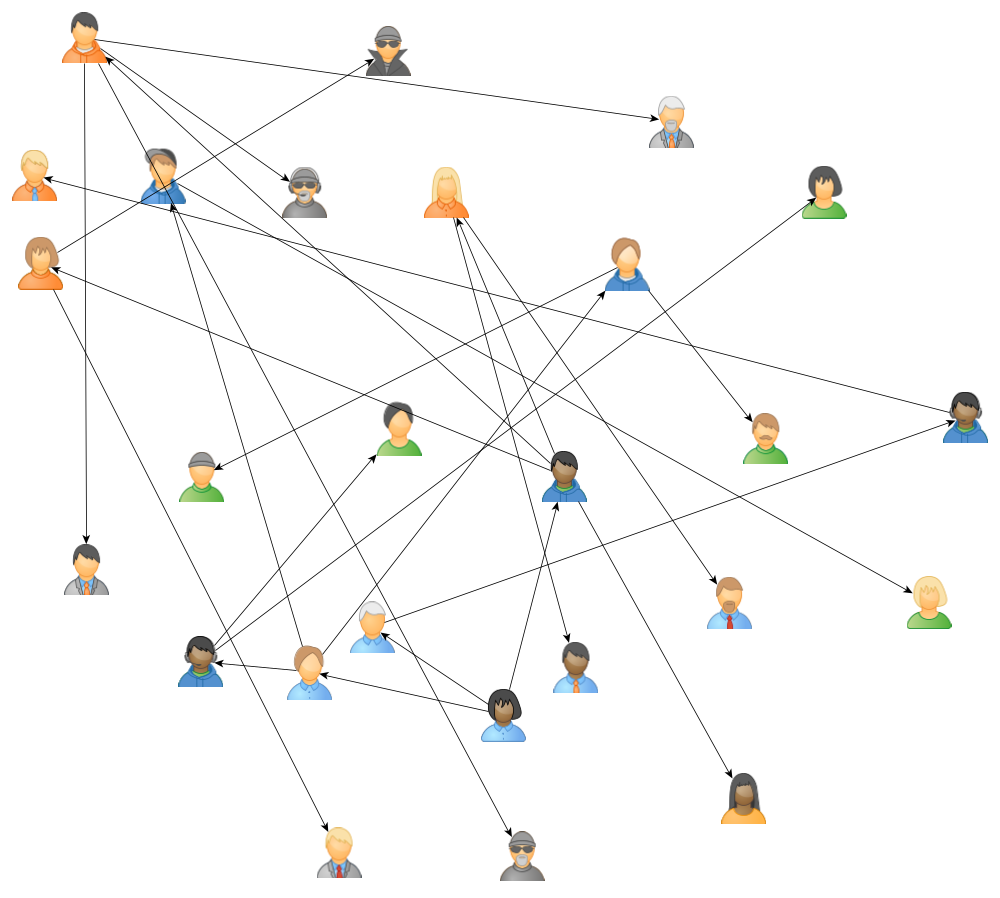
\includegraphics[width=10cm]{img/graphe2_random.png}
\end{center}
\end{frame}
\begin{frame}{Constat}
C'est le fouillis, n'est-ce pas ? \\

En déplaçant les sommets du graphe on peut le présenter ainsi :
\end{frame}
\begin{frame}{}
\begin{center}
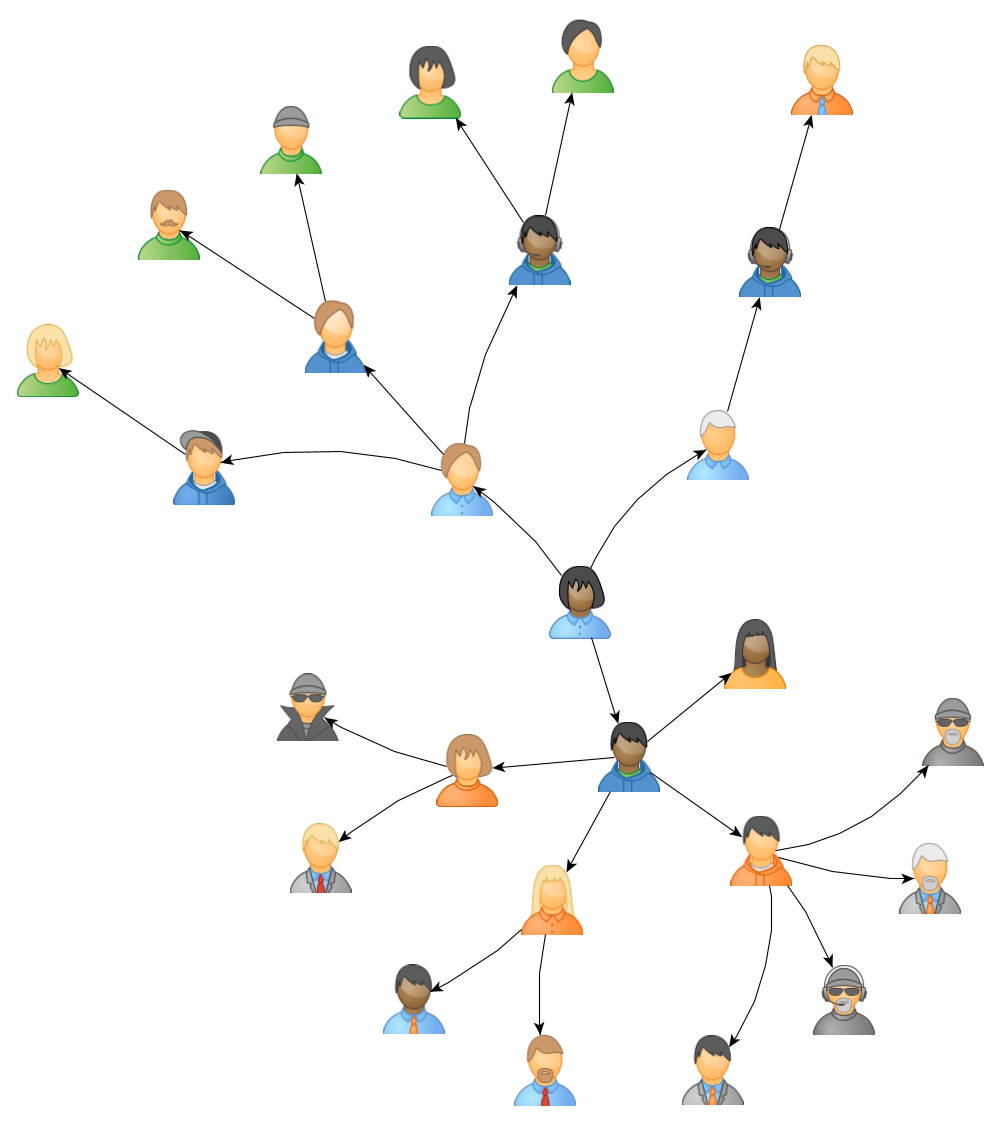
\includegraphics[width=8cm]{img/graphe2_radial.png}
\end{center}
\end{frame}
\begin{frame}{}
C'est le même graphe mais on y voit plus clair... et on y voit encore plus clair comme ça :
\end{frame}
\begin{frame}{}
\begin{center}
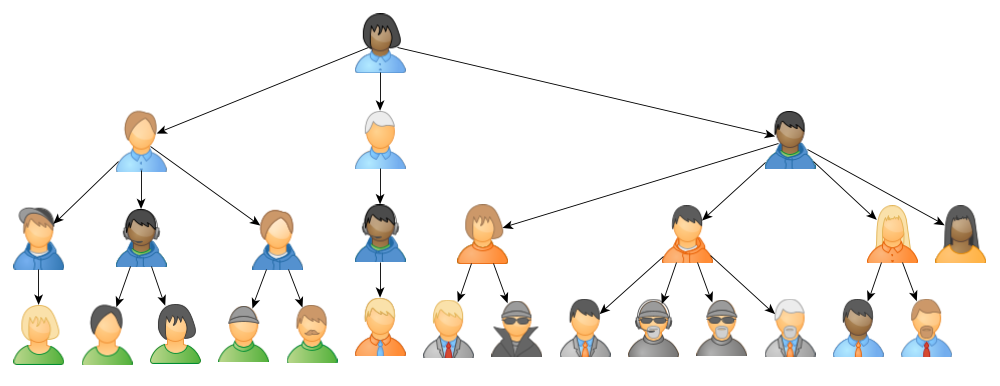
\includegraphics[width=\linewidth]{img/graphe2_tree.png}
\end{center}
On voit clairement le « patient zéro» et on reconnaît quelque chose qui ressemble à une structure que l'on a déjà rencontrée :\pause \ une arborescence.
\end{frame}
\begin{frame}{Conclusion}
La représentation graphique d'un graphe orienté ne le caractérise pas, même si certaines représentations aident à mieux en cerner la structure.\\

Ce qui caractérise un graphe orienté c'est bel et bien ses \alert{sommets} et ses \alert{arcs}.
\end{frame}
\section{Représentations d'un graphe}
\begin{frame}{Situation}
Abel, Brieuc, Corentin, David et Ewen postent des messages sur un réseau social. Un message peut-être « aimé» par n'importe quel utilisateur, y compris son créateur.\\ \pause
On regarde, sur une période de deux semaines, qui a aimé les messages de qui. Voici les résultats : \pause

\begin{enumerate}[--]
	\item 	Abel a aimé des messages de Corentin  et David;\pause
	\item 	Brieuc a aimé ses messages, ceux d'Abel et de Corentin;\pause
	\item 	Corentin a aimé les messages de David;\pause
	\item 	David a aimé ses propres messages;\pause
	\item 	Ewen a aimé les messages d'Abel.
\end{enumerate}
\end{frame}

\begin{frame}{Représentation graphique}
\begin{center}
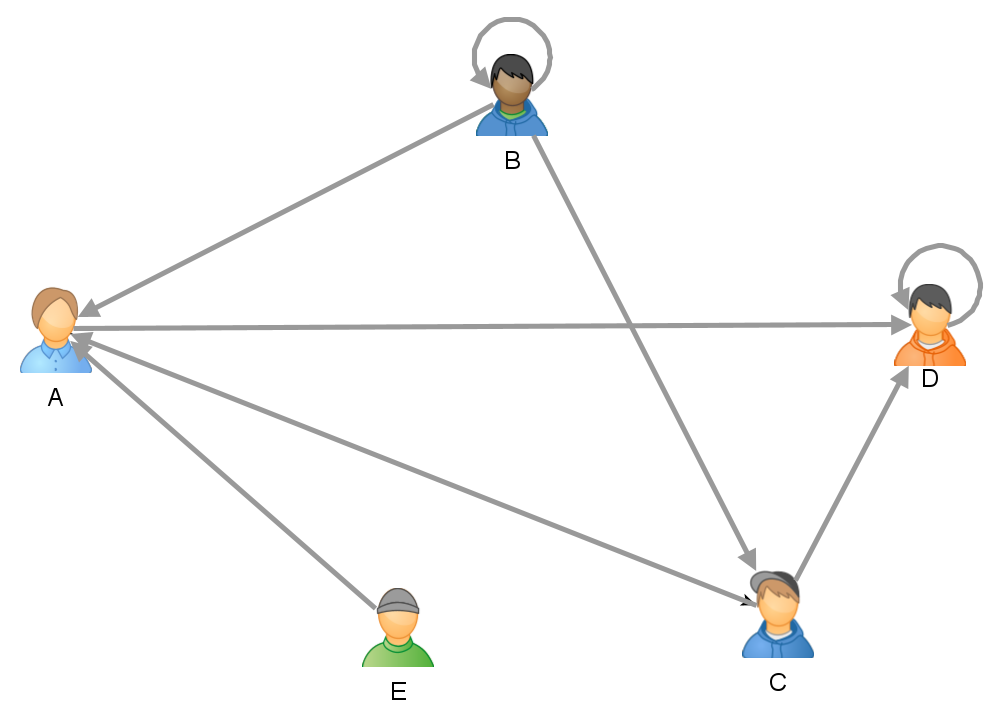
\includegraphics[width=\linewidth]{img/graphe1.png}
\end{center}
\end{frame}

\begin{frame}{Graphe orienté}
Ces résultats permettent de produire un \alert{graphe orienté} :\pause
\begin{enumerate}[--]
	\item 	les \alert{sommets du graphe} représentent les personnes;\pause
	\item 	les \alert{arcs} sont des flèches qui représentent le fait que la personne de départ aime les messages de celle d'arrivée.
\end{enumerate}
\end{frame}

\begin{frame}{Tableau de successeurs}
On peut aussi représenter les résultats dans un tableau :

\begin{center}
\begin{tabular}{|l|>{\centering\arraybackslash}p{.5cm}|>{\centering\arraybackslash}p{.5cm}|>{\centering\arraybackslash}p{.5cm}|>{\centering\arraybackslash}p{.5cm}|>{\centering\arraybackslash}p{.5cm}|}
\hline\rowcolor{UGLiBlack}
\textbf{\color{UGLiWhite}personne}& \textbf{\color{UGLiWhite}A} & \textbf{\color{UGLiWhite}B} &\textbf{\color{UGLiWhite}C}& \textbf{\color{UGLiWhite}D} & \textbf{\color{UGLiWhite}E} \\
\hline
aime les messages de  & C,D & A, B,C & D & D & A \\
\hline


%
% UGLiPurple		UGLiRed			UGLiOrange		UGLiYellow		UGLiGreen		UGLiDarkGreen	UGLiBlue	
% UGLiDarkBlue		UGLiBlack		UGLiWhite
%
% TolDarkPurple		TolDarkBlue		TolLightBlue	TolLightGreen	TolDarkGreen	TolDarkBrown	TolLightBrown	
% TolDarkRed		TolLightRed		TolLightPink	TolDarkPink		TolLightPurple
%
\end{tabular}
\end{center}
\end{frame}

\begin{frame}{Tableau de prédécesseurs}
On peut aussi recopier le tableau en donnant pour chaque personne la liste de ses « followers» (personnes qui ont aimé ses messages) :

\begin{center}
\begin{tabular}{|l|>{\centering\arraybackslash}p{1cm}|>{\centering\arraybackslash}p{1cm}|>{\centering\arraybackslash}p{1cm}|>{\centering\arraybackslash}p{1cm}|>{\centering\arraybackslash}p{1cm}|}
\hline\rowcolor{beamerBlack}
\textbf{\color{beamerWhite}personne}& \textbf{\color{beamerWhite}A} & \textbf{\color{beamerWhite}B} &\textbf{\color{beamerWhite}C}& \textbf{\color{beamerWhite}D} & \textbf{\color{beamerWhite}E} \\
\hline
followers  & B,E & B & A,B & A,C,D & --- \\
\hline
\end{tabular}
\end{center}
\end{frame}

\begin{frame}{Matrice d'adjacence}
On peut aussi présenter les données ainsi :

\begin{center}
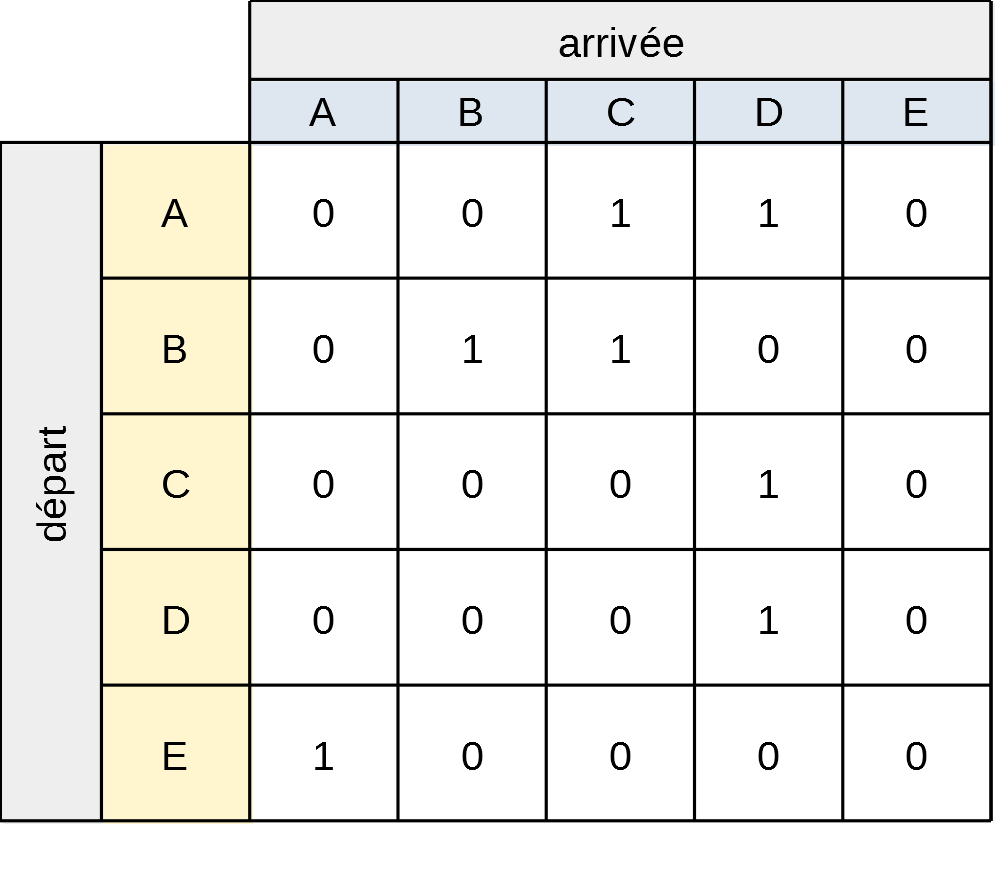
\includegraphics[width=7cm]{img/prematrice.png}
\end{center}
\end{frame}

\begin{frame}{Conclusion}
Il y a donc plusieurs manières de représenter un graphe orienté.\\\pause

À ces représentations correspondent différentes \alert{implémentations}.
\end{frame}
\section{Un peu de théorie}
\begin{frame}{Définition}
Un graphe orienté $G$, c'est la donnée de\pause
\begin{enumerate}[--]
	\item 	un ensemble $S=\{s_1;\,...;\,s_n\}$ de \alert{sommets};\pause
	\item 	un ensemble $A$ composé d'\alert{arcs} du type $(s_i;\,s_j)$, qui indiquent qu'il y a « une flèche» partant du sommet $s_i$ et allant au sommet $s_j$.:\\ $s_i$ est appelé l'\alert{origine} de l'arc et $s_j$ son \alert{extrémité}.
\end{enumerate}
\end{frame}
\begin{frame}{Exemple}
\begin{center}
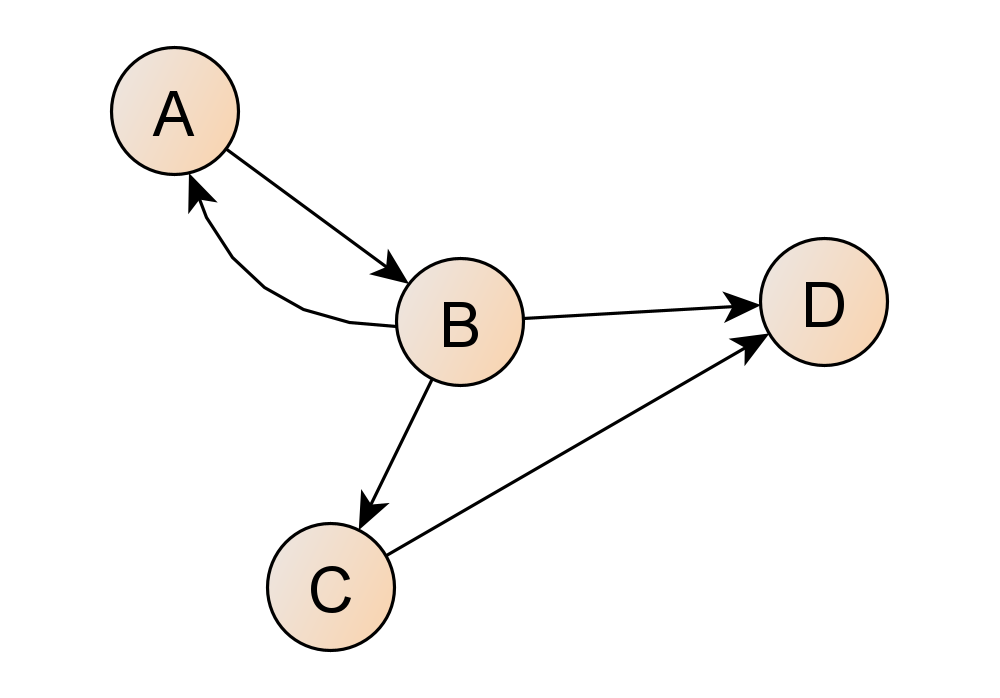
\includegraphics[width=7cm]{img/ex_graphe_oriente.png}
\end{center}
\pause
Ici l'ensemble des sommets est $\{A;\,B;\,C;\,D\}$.\\\pause

L'ensemble des arcs est $\{(A;B);\,(B;A);\,(B;C);\,(B;D);\,(C;D)\}$
\end{frame}

\begin{frame}{Exercice}
Donner l'ensemble des sommets et l'ensemble des arc du graphe suivant.
\begin{center}
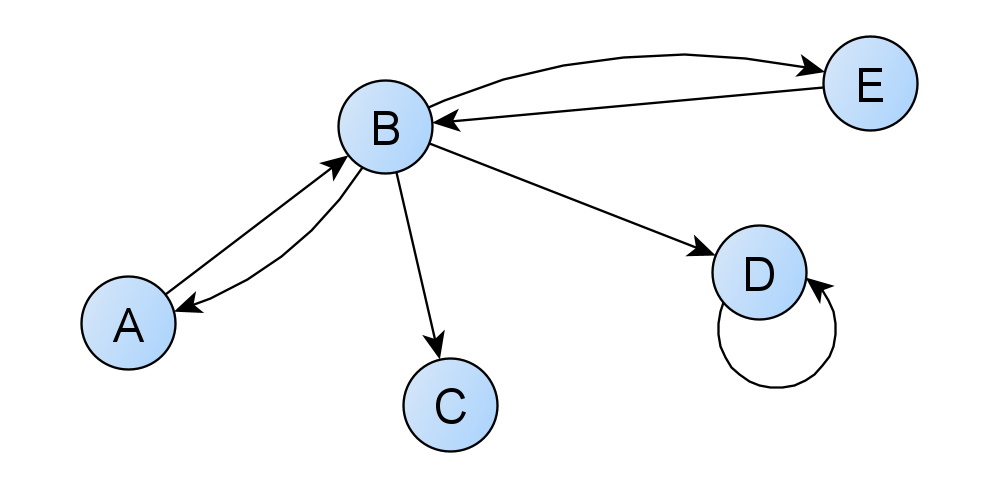
\includegraphics[width=7cm]{img/exo_graphe.png}
\end{center}
\end{frame}
\begin{frame}{Définition : boucle}
Un arc dont l'origine et l'extrémité sont confondues d'appelle une \alert{boucle}.
\end{frame}
\begin{frame}{Définition : Successeurs, prédécesseurs}
Soit un graphe de sommets $S$ et d'arcs $A$. Soit $s$ un sommet.\\\pause

On note $\Gamma^+(s)$ l'ensemble des \alert{successeurs de $s$}.\\\pause
C'est l'ensemble des extrémités des arcs \alert{partant de $s$}.\\\pause

De même, on note $\Gamma^-(s)$ l'ensemble des \alert{prédécesseurs de $s$}.\\\pause
C'est l'ensemble des origines des arcs \alert{arrivant sur $s$}.\\
\end{frame}
\begin{frame}{Successeurs : exemple}
\begin{center}
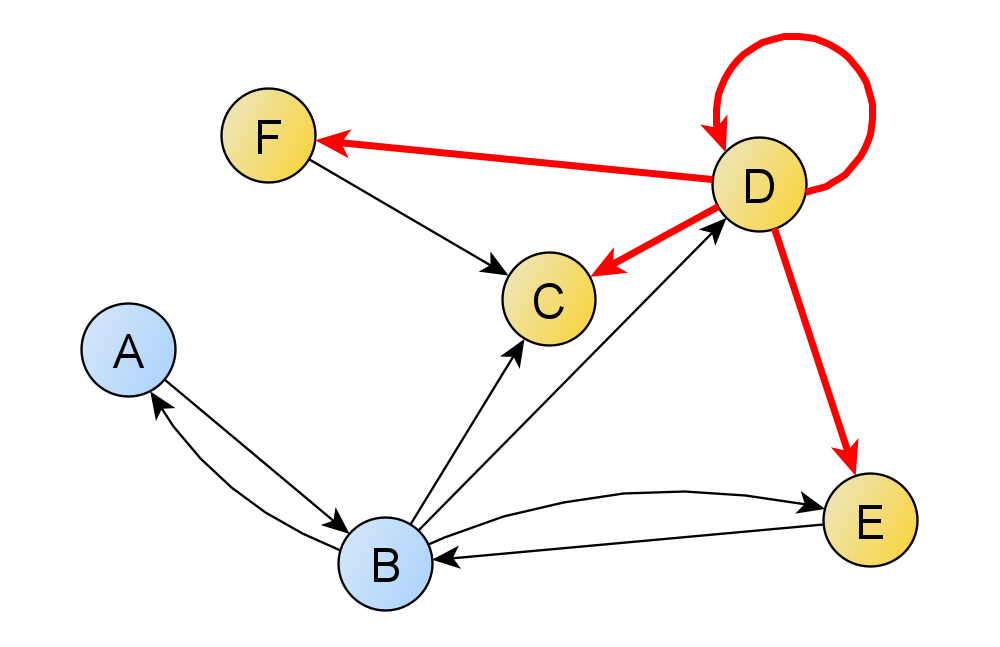
\includegraphics[width=7cm]{img/successeurs.png}
\end{center}
Dans ce graphe, il y a 4 arcs d'origine D.\pause Leurs extrémités sont les points C,D,E et F.\\\pause
Ainsi $\Gamma^+(D)=\{C;\,D;\,E;\,F\}$.
\end{frame}

\begin{frame}{Tableau des successeurs}
On peut caractériser tout graphe à partir d'un \alert{tableau des successeurs}.\\\pause

Voici celui du graphe précédent :
\begin{center}
\begin{tabular}{|c|c|c|c|c|c|c|}
\hline\rowcolor{beamerBlack}
 \textbf{\color{beamerWhite}Sommet} & \textbf{\color{beamerWhite}A} & \textbf{\color{beamerWhite}B} &\textbf{\color{beamerWhite}C}& \textbf{\color{beamerWhite}D} & \textbf{\color{beamerWhite}E}& \textbf{\color{beamerWhite}F} \\
\hline
successeurs & B & A, C, E & --- & C, D, E, F & B & C \\
\hline
\end{tabular}
\end{center}
\end{frame}
\begin{frame}{Prédécesseurs : exemple}
\begin{center}
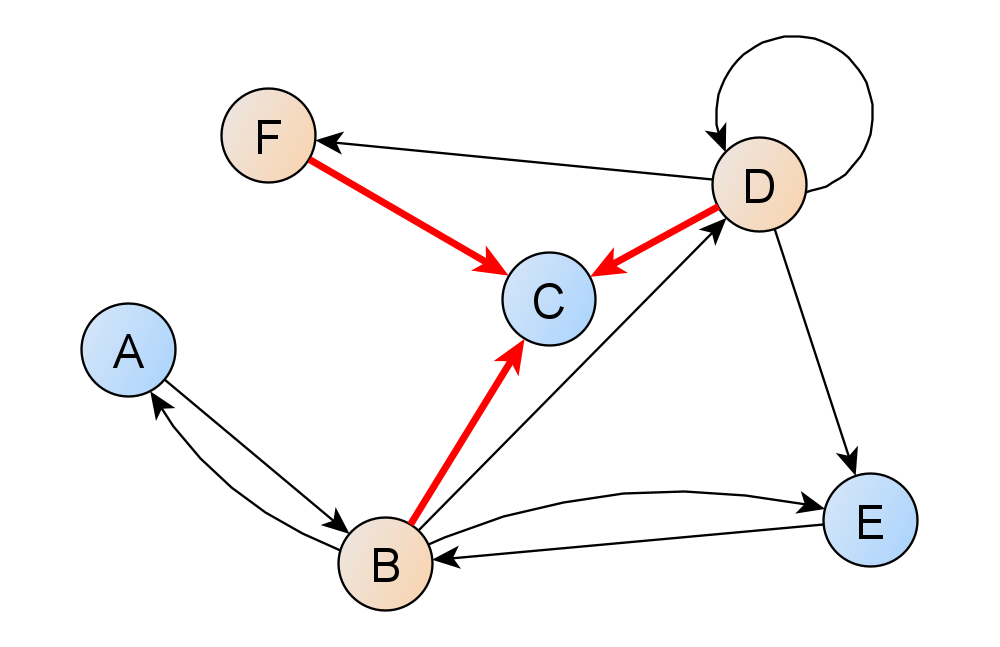
\includegraphics[width=7cm]{img/predecesseurs.png}
\end{center}
Dans ce graphe, il y a 3 arcs d'extrémité C.\\ \pause
Leurs origines sont les points B,D et F.\\\pause
Ainsi $\Gamma^-(C)=\{B;\,D;\,F\}$.
\end{frame}
\begin{frame}{Tableau des prédécesseurs}
Il caractérise également le graphe. Voici celui du graphe précédent :
\begin{center}
\begin{tabular}{|c|c|c|c|c|c|c|}
\hline\rowcolor{beamerBlack}
\textbf{\color{beamerWhite}Sommet} & \textbf{\color{beamerWhite}A} & \textbf{\color{beamerWhite}B} &\textbf{\color{beamerWhite}C}& \textbf{\color{beamerWhite}D} & \textbf{\color{beamerWhite}E}& \textbf{\color{beamerWhite}F} \\
\hline
prédécesseurs & B & A, E & B, D, F & B, D & B, D & D \\
\hline
\end{tabular}
\end{center}
\end{frame}
\section{Matrice d'adjacence}
\begin{frame}{Définition}
Soit un graphe G de sommets  $S=\{s_1;\,...;\,s_n\}$ et d'arcs A.\\\pause 
On appelle \textit{matrice d'adjacence de} G la matrice carrée d'ordre n $M=(m_{ij})$ telle que \pause
\begin{enumerate}[--]
	\item 	$m_{ij}=1$ s'il y a un arc partant de $s_i$ et arrivant sur $s_j$;\pause
	\item 	$m_{ij}=0$ sinon.\pause
\end{enumerate}
$i$ est le numéro de ligne et $j$ celui des colonnes de la matrice $M$.
\end{frame}
\begin{frame}{Exemple}
\begin{center}
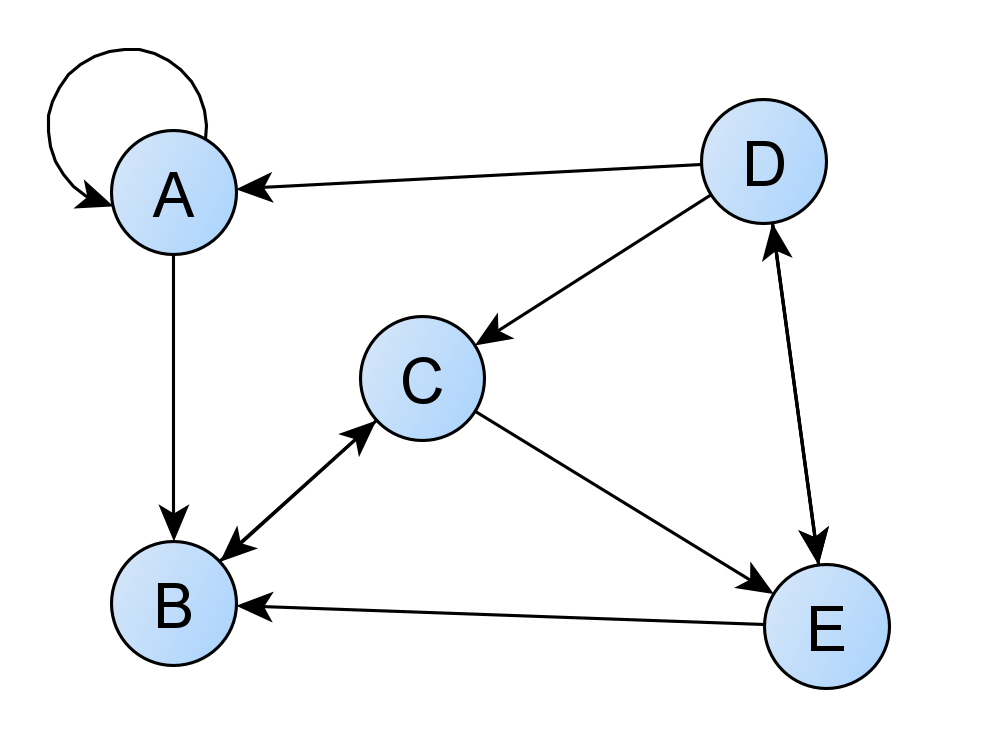
\includegraphics[width=3.5cm]{img/matr_adj1.png}
\end{center}
En écrivant les sommets dans l'ordre alphabétique, on obtient\pause
$$\scriptsize M=\begin{pmatrix}
1 &1 &0 & 0&0  \\
0 & 0&1 &0 &0  \\
0 & \boxed{1} & 0 & 0 & 1\\
1 & 0 & 1 & 0 & 1\\
0 & 1 & 0 &{\color{red}1} & 0 
\end{pmatrix}$$
L'élément encadré de $M$ est à la 3\eme ligne et à la 2\eme colonne : c'est $m_{32}$.\pause Il vaut 1 et signifie qu'il y a un arc partant du sommet 3, donc C, et allant au sommet 2, donc B.\\\pause
De même, du 5\eme sommet E, il existe un arc allant vers le 4\eme (D), donc $m_{54}=1$ (en rouge).\pause
\end{frame}
\begin{frame}{Remarque}
Dans une matrice d'adjacence\pause
\begin{enumerate}[--]
	\item 	Les lignes correspondent aux points de départ, les colonnes au point d'arrivée;\pause
	\item 	Sur une ligne donnée(la i\eme par exemple), on peut lire \textit{tous les successeurs} de $s_i$;\pause
	\item 	Sur une colonne donnée, (la j\eme par exemple), on lit \textit{tous les prédécesseurs} de $s_j$;
\end{enumerate}
\end{frame}
\section*{Chemins, circuits}
\begin{frame}{Définitions}
On considère un graphe orienté.\\

Un \alert{chemin} est une succession de sommets dans un ordre donné, chacun étant relié au suivant par un arc.\\

La \alert{longueur} du chemin, c'est le nombre d'arcs qui composent le chemin.\\
C'est aussi le nombre de sommets qui composent le chemin moins un.
\end{frame}
\begin{frame}{Exemple}
\begin{center}
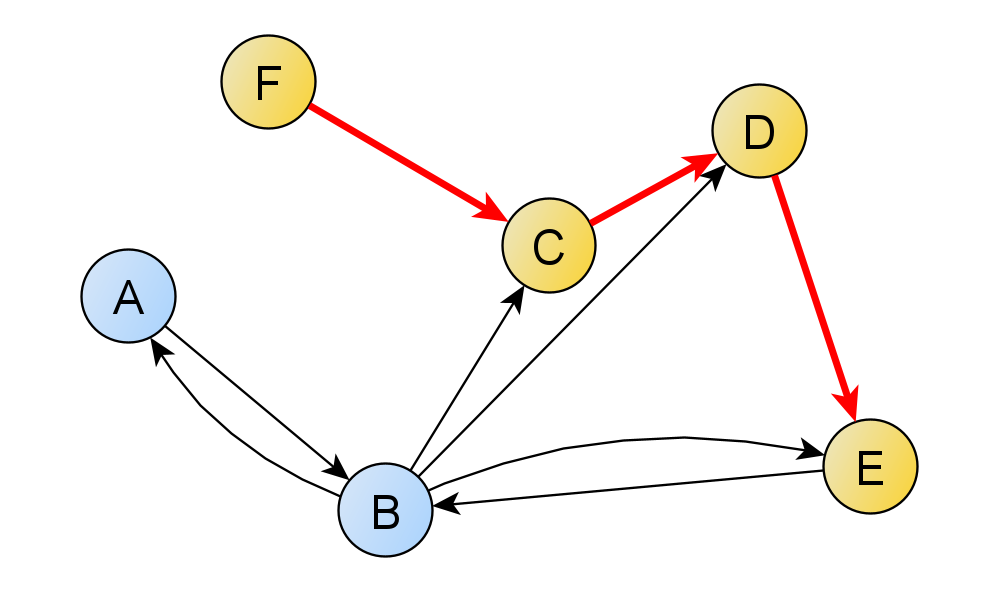
\includegraphics[width=7cm]{img/chemin.png}
\end{center}
$(F,\,C,\,D,\,E)$ est un chemin de longueur 3.\\

$(F,\,C,\,B,\,E)$ n'en est pas un car l'arc $(C,\,B)$ n'existe pas. 
\end{frame}
\begin{frame}{Circuit}
Un \alert{circuit} est un chemin dont le premier et le dernier sommet sont identiques (un chemin « fermé» en quelque sorte).
\begin{center}
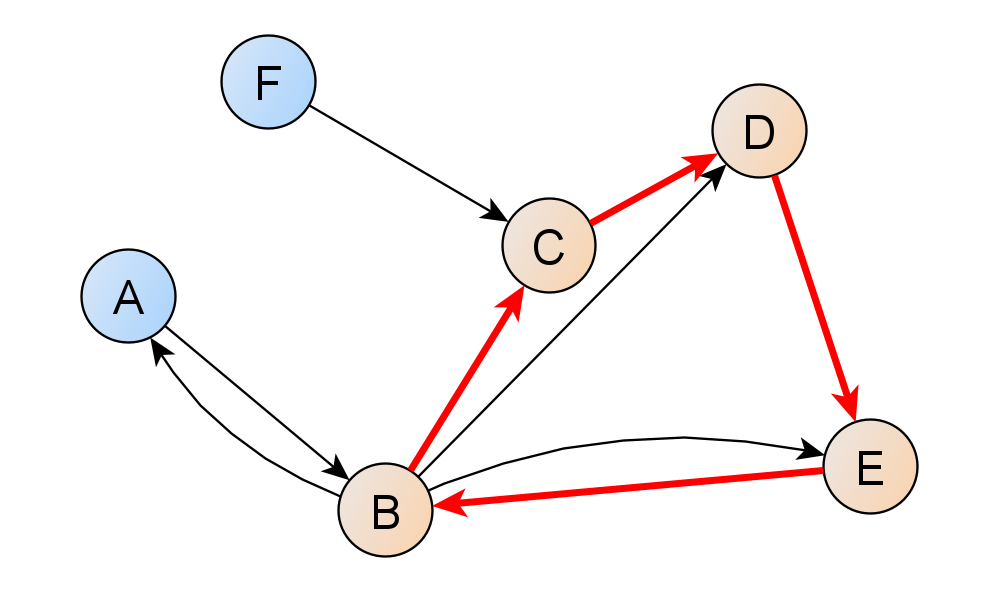
\includegraphics[width=7cm]{img/circuit.png}
\end{center}
$(C,\,D,\,E,\,B,\,C)$ est un circuit de longueur 4.
\end{frame}
\section*{Implémentation n°1}
\begin{frame}[fragile]{À l'aide d'une matrice d'adjacence}
\begin{center}
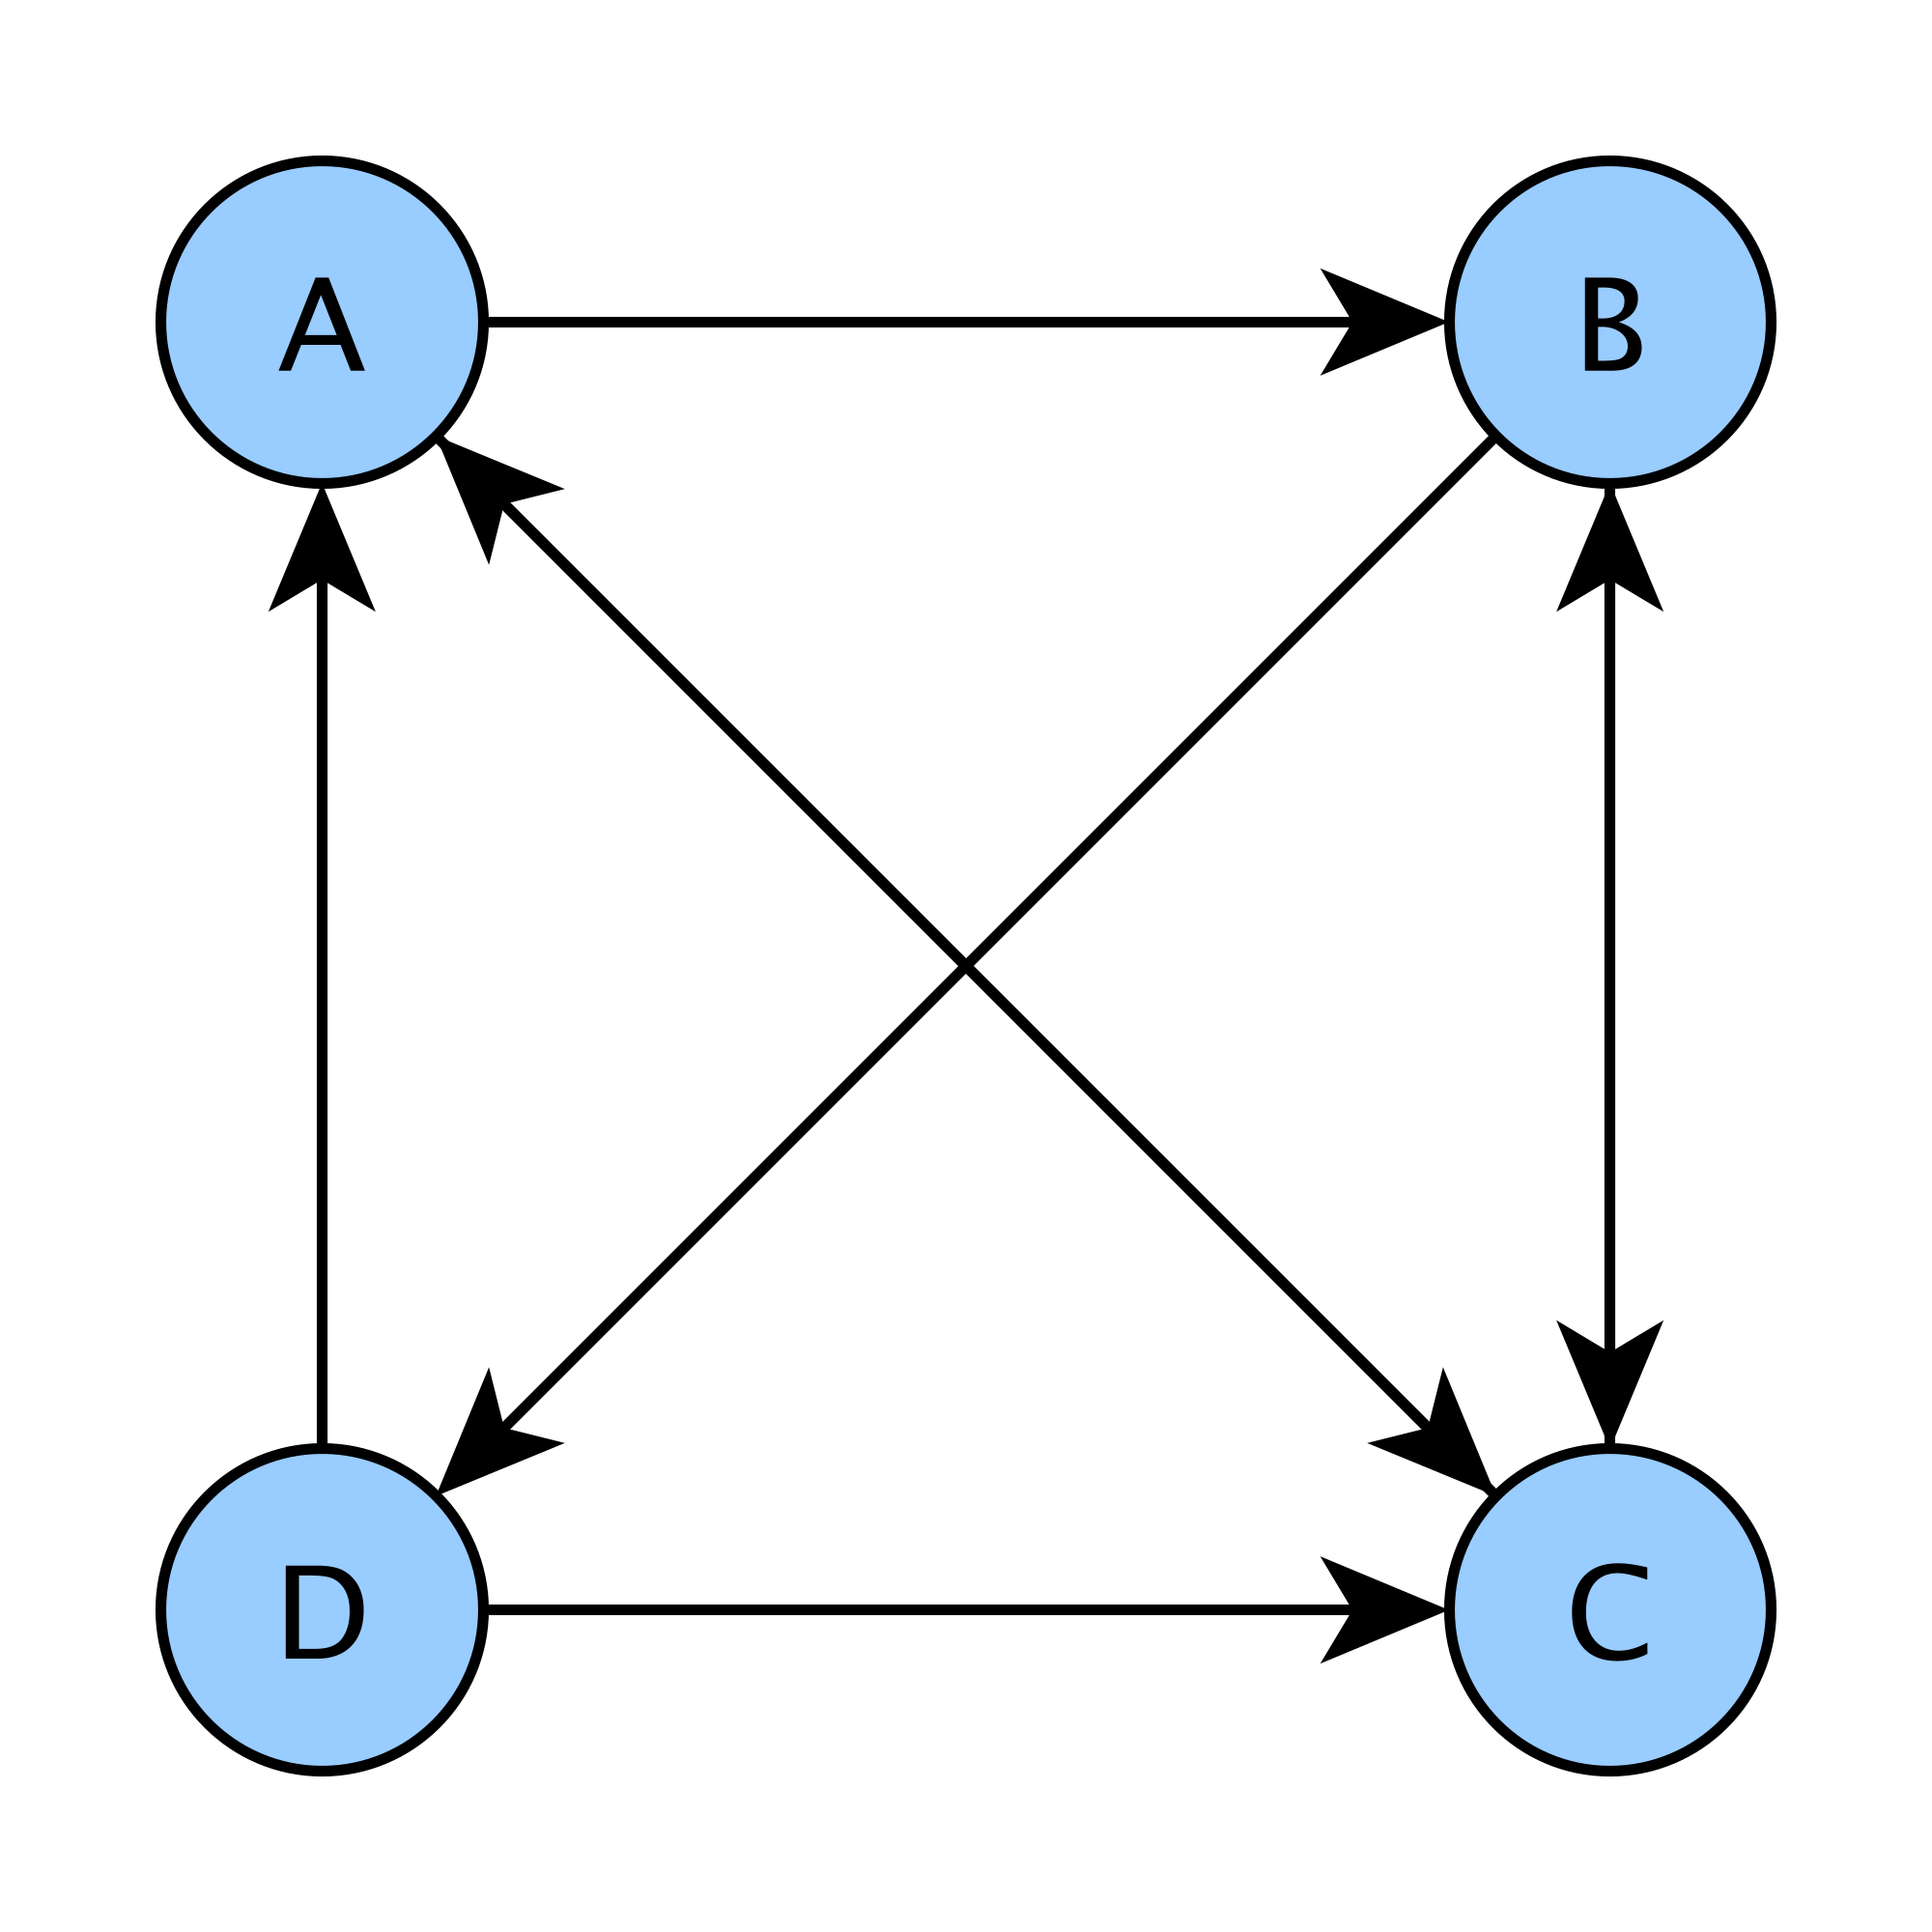
\includegraphics[width=5cm]{img/graphe_matrice}
\end{center}
\begin{minted}{python}
G = [[0, 1, 1, 0], # successeurs de A
     [0, 0, 1, 1], # successeurs de B
     [1, 1, 0, 0], # successeurs de C
     [1, 0, 1, 0]] # successeurs de D
\end{minted}
\end{frame}
\begin{frame}{Intérêts}
\begin{enumerate}[--]
	\item 	Très simple à mettre en \oe uvre.
	\item 	Fonctions \mintinline{python}{successeurs} et \mintinline{python}{arc} facile à coder.
\end{enumerate}
\end{frame}
\begin{frame}{Inconvénients}
\begin{enumerate}[--]
	\item 	On ne peut pas facilement ajouter d'autres sommets.
	\item 	Pour $n$ sommets on a une matrice $n\times n$, ce qui prend beaucoup de place surtout s'il n'y a pas beaucoup d'arcs.
    \item 	On n'a pas les noms des sommets dans la matrice, c'est à nous de connaître la correspondance.
\end{enumerate}
\end{frame}
\begin{frame}{Remarques}
\begin{enumerate}[--]
	\item 	On peut très facilement encapsuler la matrice et les fonctions dans une classe.
	\item 	Attention, en \textsc{Python}, les indices commencent à 0, donc il y a un petit « décalage» par rapport à la matrice théorique.	
\end{enumerate}

\end{frame}
\section*{Implémentation n°2}
\begin{frame}[fragile]{Dictionnaire d'adjacence}
\begin{center}
	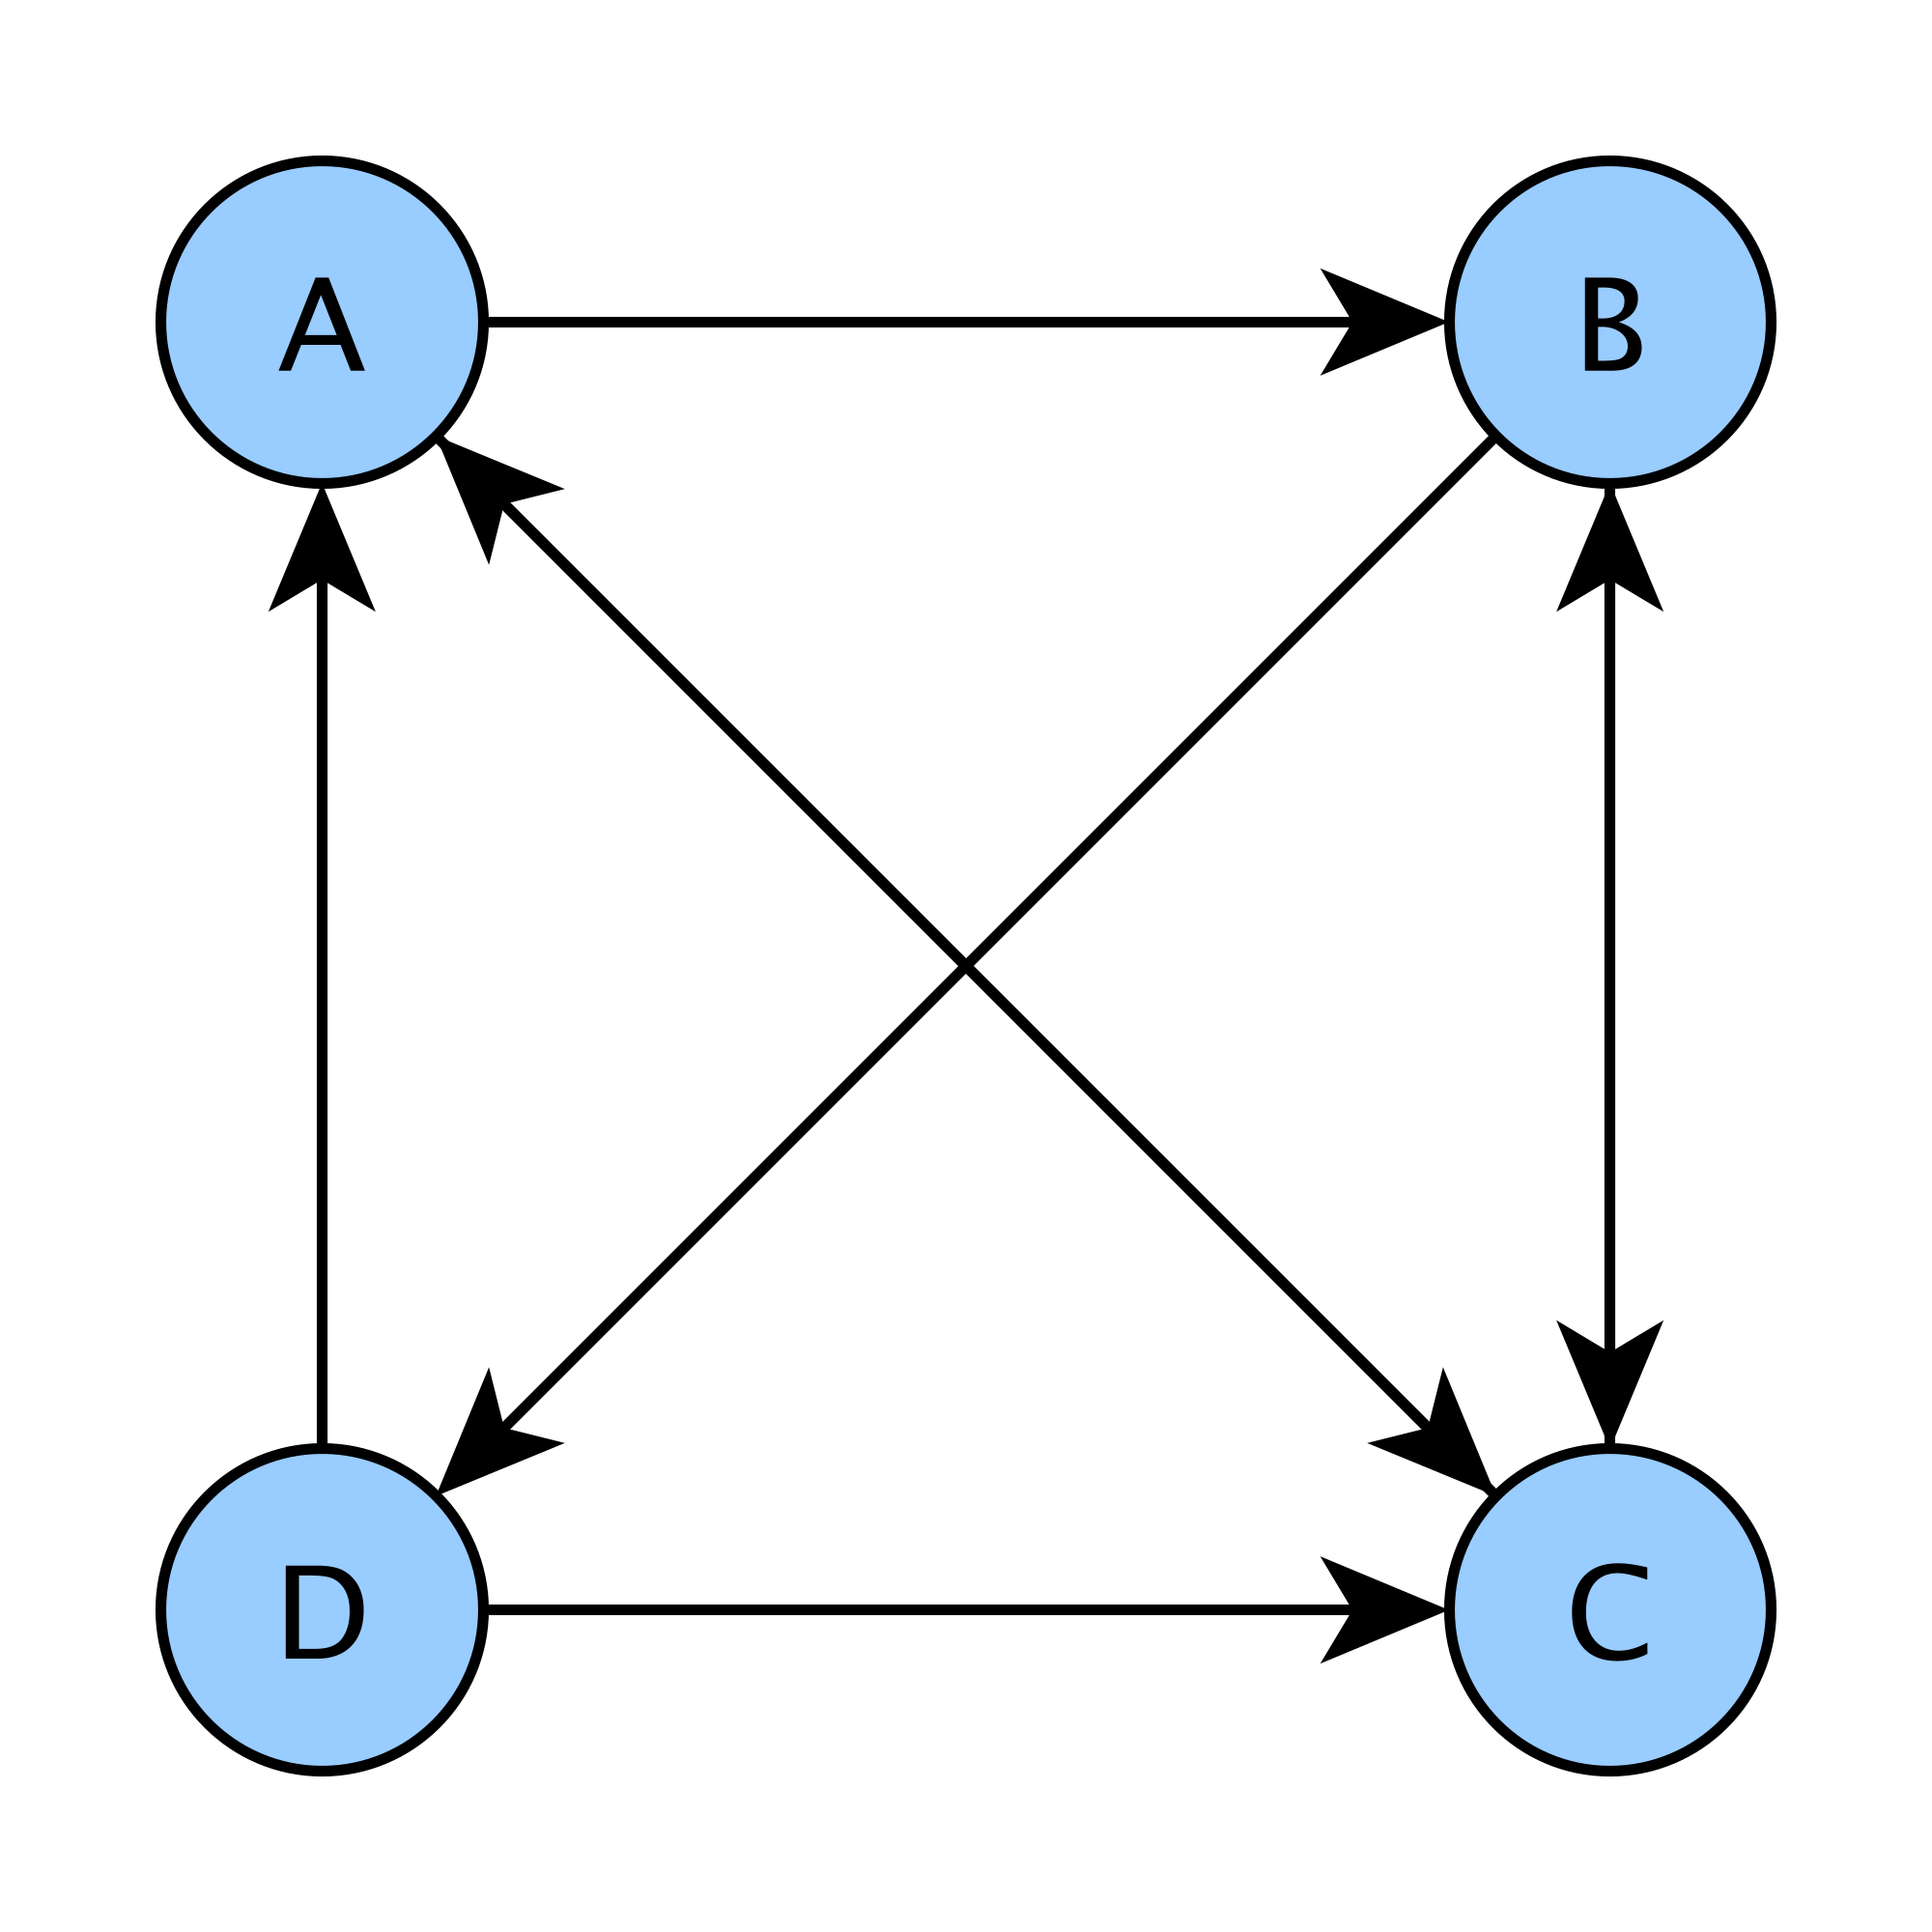
\includegraphics[width=5cm]{img/graphe_matrice}
\end{center}
\begin{minted}{python}
G = {'A' : ['B','C'], # les sommets sont les clés
     'B' : ['C','D'], # et les valeurs les listes 
     'C' : ['A','B'], # des successeurs de chaque
     'D' : ['A','C']} # clé
\end{minted}
\end{frame}

\begin{frame}{Intérêts}
\begin{enumerate}[--]
    \item On peut facilement ajouter d'autres sommets.
    \item On dispose des noms des sommets.
    \item Solution assez « élégante ».
\end{enumerate}
\end{frame}
\begin{frame}{Inconvénients}
    Si le nombre de sommets (et surtout d'arcs) est grand, cette implémentation prendra beaucoup plus de place en mémoire qu'une simple matrice d'adjacence.
\end{frame}

\begin{frame}{Remarque}
Encore une fois, il est judicieux d'encapsuler ce dictionnaire dans une classe.\\ 
On pourra alors définir des méthodes telles que :
\begin{enumerate}[--]
	\item 	\texttt{liste\_sommets}
	\item 	\texttt{successeurs}
    \item 	\texttt{predecesseurs}
    \item 	\textit{Et c\ae tera}
\end{enumerate}
\end{frame}
\end{document}